%%%%%%%%%%%%%%%%%%%%%%%%%%%%%%%%%%%%%%%%%%%
%%%%%%%%%%%%%%%%%%%%%%%%%%%%%%%%%%%%%%%%%%%
%%%%%%%%%%%%%%% CHAPTER 03 %%%%%%%%%%%%%%%%


\section{Sensoriamento e atuadores}

\frame{
\frametitle{Sensores}
\begin{block}{Contextualização}
O velocímetro de um automóvel indica a velocidade de deslocamento porque existe um \textbf{sensor} que é capaz de medir a velocidade das rodas.
\end{block}
\centerline{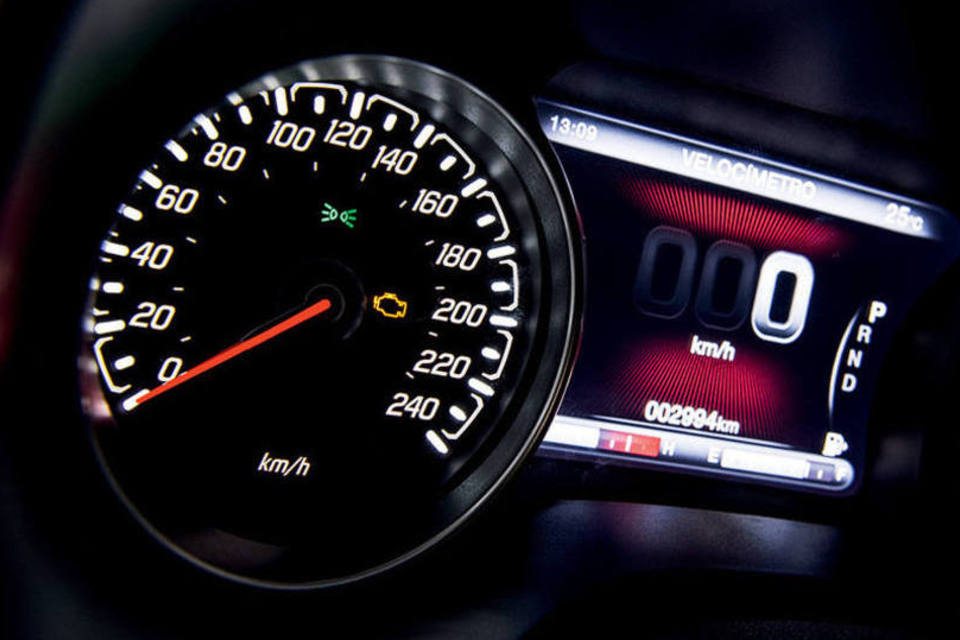
\includegraphics[width=0.7\linewidth]{Figuras/Ch03/fig1.jpeg}}
}

\frame{
\frametitle{Sensores}
\begin{block}{Contextualização}
A porta de uma geladeira ao ser
aberta acende a luz, porque há um \textbf{sensor} que indica que ela foi aberta.
\end{block}
\centerline{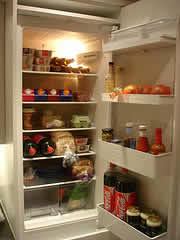
\includegraphics[width=0.3\linewidth]{Figuras/Ch03/fig2.jpg}}
}

\frame{
\frametitle{Sensores}
\centerline{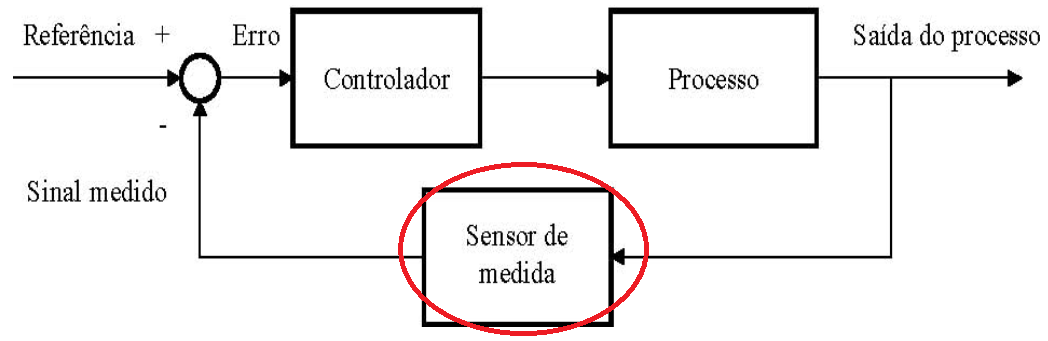
\includegraphics[width=0.9\linewidth]{Figuras/Ch03/fig3.PNG}}
\begin{block}{Definição}
É um dispositivo capaz de \textbf{monitorar a variação de uma grandeza física} e transmitir esta informação a um sistema em que a indicação seja inteligível para nós ou para o elemento de controle do sistema.
\end{block}
}

\frame{
\frametitle{Transdutores}
\begin{block}{Definição}
Todos os dispositivos sensores são compostos por elementos denominados \textbf{transdutores}, pois são capazes de \textbf{transformar um tipo de energia em outro}. A maior parte dos sensores é constituída por transdutores que convertem uma grandeza de entrada em uma \textbf{grandeza elétrica}, que pode ser processada por um circuito elétrico ou eletrônico.
\begin{itemize}
    \item Transdutor: é todo dispositivo que recebe um sinal de entrada na forma de uma grandeza física, e fornece uma resposta na saída, da mesma espécie ou diferente, que reproduz certas características do sinal de entrada a partir de uma relação definida.
\end{itemize}
\end{block}
}

\frame{
\frametitle{Tipos de sinais}
\begin{block}{Definição}
\begin{itemize}
    \item Os sensores podem ser classificados segundo o \textbf{tipo de sinal} que transformam. Assim, para estudar sensores é necessário começar pelos tipos de sinais.
\end{itemize}
Um sinal é uma \textbf{informação} na forma de um valor (ou de uma curva de valores) de uma grandeza física.
\end{block}
}

\frame{
\frametitle{Tipos de sinais}
\begin{block}{Sinal digital}
\begin{itemize}
    \item O \textbf{sinal digital binário} só pode assumir \textbf{dois valores}. 
    \item Estes valores são associados a
    \textbf{estados} que podem indicar, por exemplo, se uma pressão está acima ou abaixo de uma determinada referência. 
    \item O valor 0 (\textbf{zero}) é geralmente utilizado para indicar estados como “falso”, “aberto”, “desligado” ou “abaixo da referência”.
    \item O valor 1 (\textbf{um}) pode
    indicar estados como “verdadeiro”, “fechado”, “ligado” ou “acima da referência”.
\end{itemize}
\end{block}
}

\frame{
\frametitle{Tipos de sinais}
\centerline{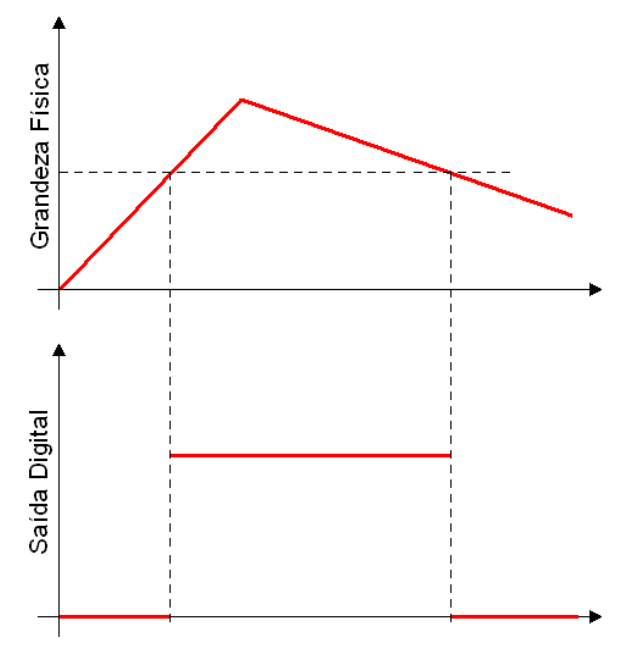
\includegraphics[width=0.6\linewidth]{Figuras/Ch03/fig4.PNG}}
}

\frame{
\frametitle{Tipos de sinais}
\centerline{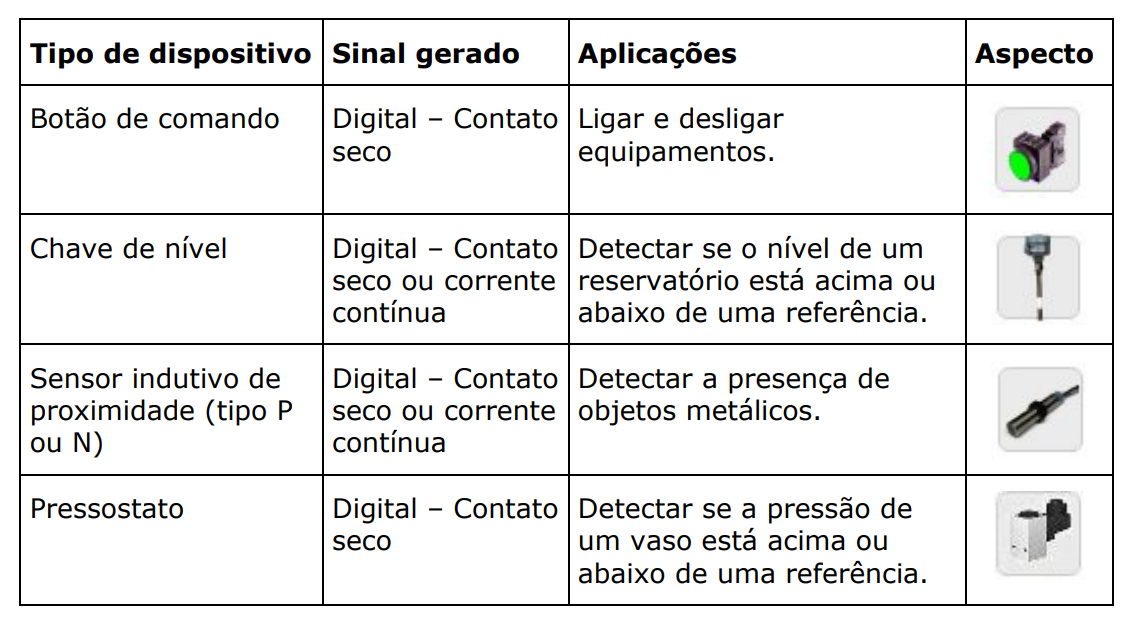
\includegraphics[width=1.1\linewidth]{Figuras/Ch03/fig5.PNG}}
}

\frame{
\frametitle{Tipos de sinais}
\begin{block}{Sinal analógico}
\begin{itemize}
    \item Um \textbf{sinal analógico} é um sinal
    \textbf{contínuo} que representa a evolução de uma grandeza, de uma variável e que apresenta \textbf{infinitos valores} mesmo que estes valores estejam em uma faixa determinada. 
    \item Vamos nos imaginar medindo o nível de um reservatório e que este nível pode variar de 0 a 10 metros de altura. Há infinitos valores de nível nesta faixa e um sinal analógico, por ser contínuo, pode representar todos estes valores. Por exemplo, o nível do reservatório pode ser de 2 metros, de 3,5 metros, de 9,75 metros, ou seja, qualquer valor entre 0 e 10 metros.
\end{itemize}
\end{block}
}

\frame{
\frametitle{Tipos de sinais}
\centerline{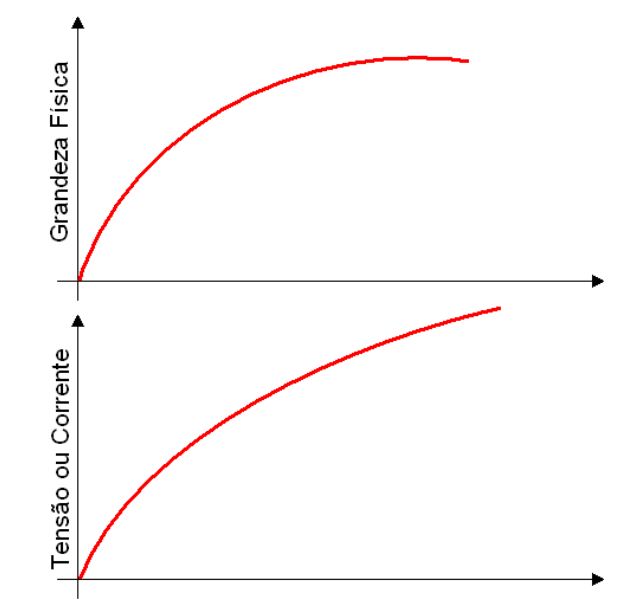
\includegraphics[width=0.6\linewidth]{Figuras/Ch03/fig6.PNG}}
}

\frame{
\frametitle{Tipos de sinais}
\centerline{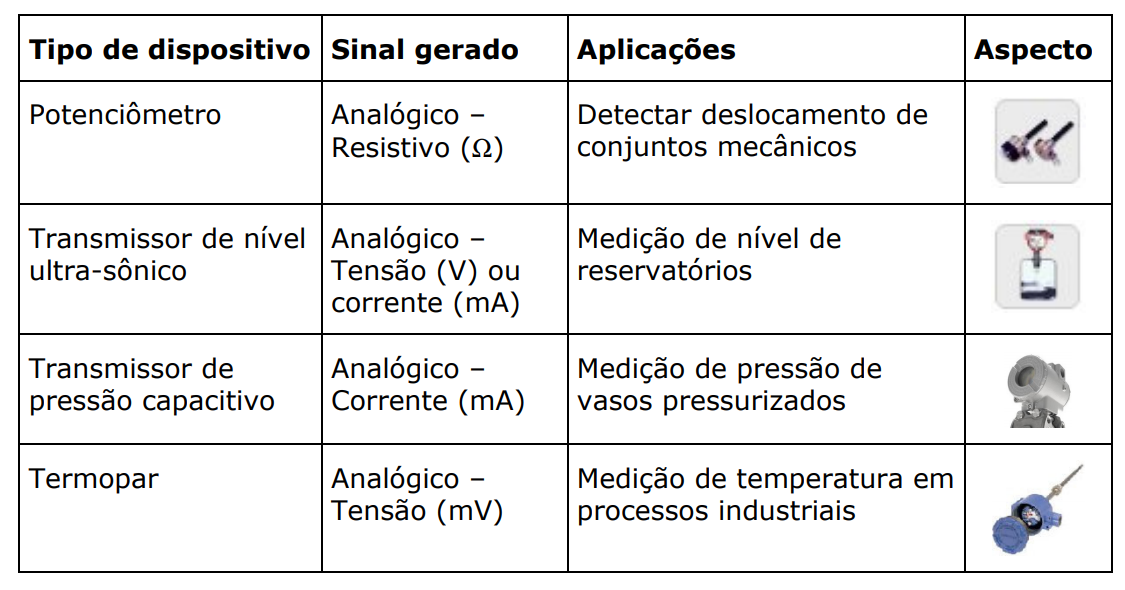
\includegraphics[width=1.1\linewidth]{Figuras/Ch03/fig7.PNG}}
}

\frame{
\frametitle{Características}
\begin{block}{Linearidade}
Esse conceito se aplica a \textbf{sensores analógicos}. É a curva de saída do sensor a partir da grandeza medida. Buscam-se \textbf{respostas proporcionais às entradas} (lineares), para facilitar a montagem do circuito de interface, porém \textbf{nem sempre isso é possível}, pois alguns sensores não são lineares. 
\end{block}
\centerline{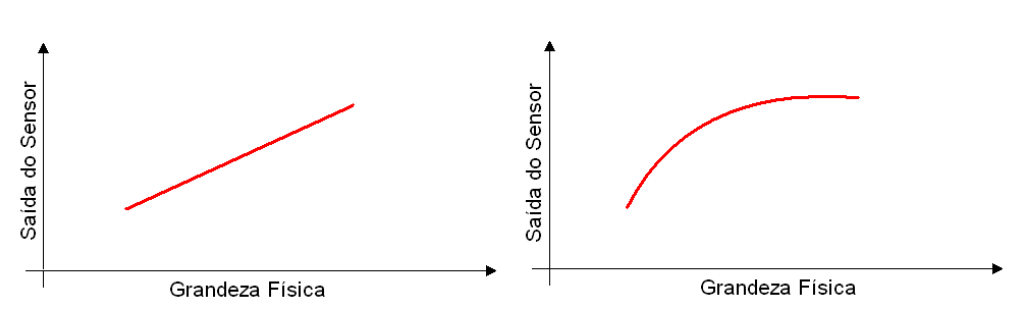
\includegraphics[width=1.1\linewidth]{Figuras/Ch03/fig8.PNG}}
}

\frame{
\frametitle{Características}
\begin{block}{Alcance (Range)}
Representa \textbf{toda a faixa de valores de entrada} de um sensor.
\end{block}
}

\frame{
\frametitle{Características}
\begin{block}{Velocidade de resposta}
Trata-se da \textbf{velocidade com que o sensor fornece o valor da variável}. O ideal é que o sensor possua uma resposta instantânea, pois uma resposta lenta pode prejudicar muito a eficiência do sistema de controle.
\end{block}
}

\frame{
\frametitle{Características}
\begin{block}{Repetibilidade}
É a habilidade do sensor de \textbf{detectar o
mesmo objeto à mesma distância, todas as vezes}.
Expresso como um percentual da distância sensora
nominal, esse número é baseado em uma temperatura ambiente constante e tensão da fonte.
\end{block}
}

\frame{
\frametitle{Sensores mecânicos}
\begin{block}{Chaves de fim de curso}
Uma chave fim de curso é um dispositivo
eletromecânico que consiste de um atuador
mecanicamente conectado a um conjunto de contatos. Podem determinar a presença ou ausência, passagem, posicionamento e término do curso de um objeto, por isso o nome de ``chave fim de curso''.
\end{block}
\centerline{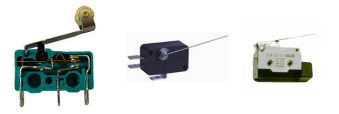
\includegraphics[width=0.9\linewidth]{Figuras/Ch03/fig9.PNG}}
}

\frame{
\frametitle{Sensores mecânicos}
\begin{block}{Chaves de fim de curso}
O tipo de sensor utilizado na porta da geladeira para acender e apagar a lâmpada é um detector de contato. 
\end{block}
\centerline{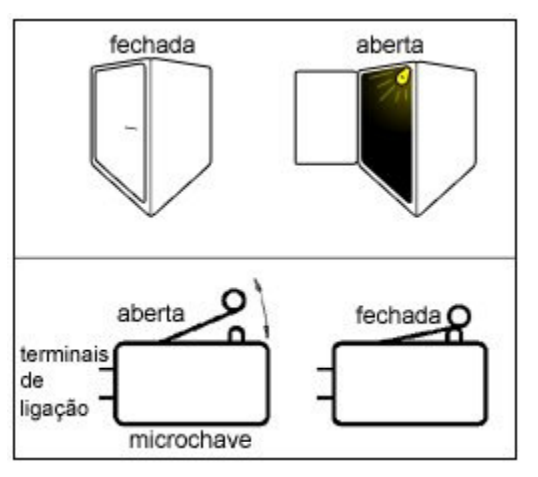
\includegraphics[width=0.5\linewidth]{Figuras/Ch03/fig10.PNG}}
}

\frame{
\frametitle{Sensores mecânicos}
\begin{block}{Chaves de fim de curso}
Outra aplicação possível é na \textbf{contagem e detecção de peças}.
\end{block}
\centerline{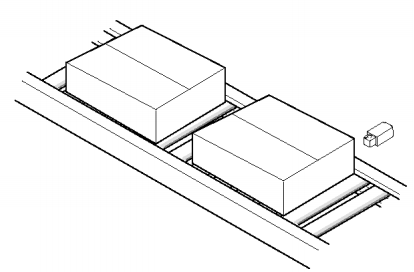
\includegraphics[width=0.7\linewidth]{Figuras/Ch03/fig11.PNG}}
}

\frame{
\frametitle{Sensores mecânicos}
\begin{block}{Chaves de fim de curso}
\textbf{Vantagens}:
\begin{itemize}
    \item Fácil utilização.
    \item Operação visível simples.
    \item Alta resistência para diferentes condições de ambiente.
    \item Alta repetibilidade.
\end{itemize}
\vspace{0.3cm}
\textbf{Desvantagens}:
\begin{itemize}
    \item Vida de contato mais curta do que as
    tecnologias de estado sólido.
    \item Peças mecânicas móveis podem apresentar desgaste.
    \item Nem todas as aplicações podem usar detecção por contato.
\end{itemize}
\end{block}
}

\frame{
\frametitle{Sensores mecânicos}
\begin{block}{Reed-Switch}
São chaves acionadas por \textbf{campo magnético}.
\end{block}
\centerline{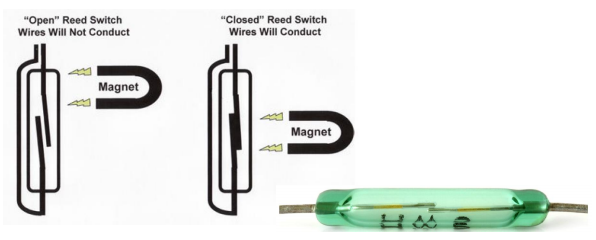
\includegraphics[width=0.9\linewidth]{Figuras/Ch03/fig12.PNG}}
}

\frame{
\frametitle{Sensores mecânicos}
\begin{block}{Reed-Switch}
Para proteger uma porta, uma janela ou um objeto qualquer contra a abertura ou remoção o que se faz é prender o ímã na parte móvel (porta, janela ou objeto) e o reed-switch na parte fixa (batente ou mesa).
\begin{itemize}
    \item O circuito deve ser projetado para operar no modo NF (Normalmente Fechado), ou seja, o circuito permanece desligado quando o reed-switch está fechado, ou com o ímã próximo.
    \item Quando o ímã é afastado, o reed-switch abre e com isso o circuito é ativado, disparando um \textbf{alarme} ou sistema de aviso.
\end{itemize}
\end{block}
\centerline{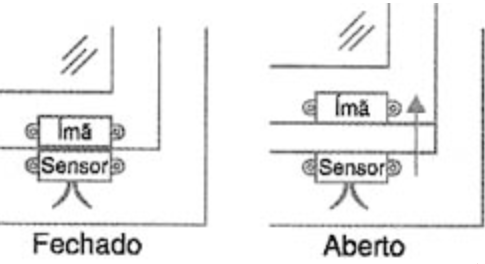
\includegraphics[width=0.5\linewidth]{Figuras/Ch03/fig13.PNG}}
}

\frame{
\frametitle{Sensores mecânicos}
\begin{block}{Reed-Switch}
\textbf{Vantagens}:
\begin{itemize}
    \item Fácil utilização.
    \item Barato.
    \item Alta velocidade de resposta.
\end{itemize}
\vspace{0.3cm}
\textbf{Desvantagens}:
\begin{itemize}
    \item Fragilidade mecânica.
    \item Susceptibilidade em gerar falso alarme.
    \item Consumo excessivo que reduz a vida útil da bateria.
\end{itemize}
\end{block}
}

\frame{
\frametitle{Sensores indutivos}
\begin{block}{}
Um sensor indutivo é usado para \textbf{detectar a presença de objetos metálicos}. O seu funcionamento é baseado, de acordo com sua característica física no \textbf{princípio da variação da indutância eletromagnética}. Ao energizar a bobina cria-se o campo eletromagnético.
\begin{itemize}
    \item Quando se introduz um objeto metálico na região ativa do sensor ocorre a detecção do objeto. Instantaneamente, o sinal da saída do sensor, que é um \textbf{sinal digital}, é modificado enviando a informação para o circuito ou para entrada digital de um equipamento que irá processá-la, como um CLP, por exemplo.
\end{itemize}
\end{block}
}

\frame{
\frametitle{Sensores indutivos}
\centerline{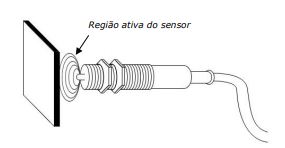
\includegraphics[width=0.8\linewidth]{Figuras/Ch03/fig14.PNG}}
}

\frame{
\frametitle{Sensores indutivos}
\begin{block}{}
\textbf{Vantagens}:
\begin{itemize}
    \item Não são afetados pela umidade.
    \item Não são afetados pelos ambientes com poeira/sujeira.
    \item Sem partes móveis/sem desgaste mecânico.
    \item Não dependem de cor.
\end{itemize}
\vspace{0.3cm}
\textbf{Desvantagens}:
\begin{itemize}
    \item Detectam somente a presença de alvos metálicos.
    \item Podem ser afetados por campos eletromagnéticos fortes.
\end{itemize}
\end{block}
}

\frame{
\frametitle{Sensores indutivos}
\centerline{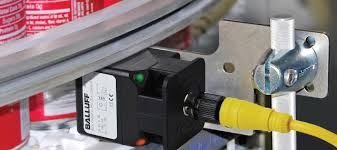
\includegraphics[width=0.9\linewidth]{Figuras/Ch03/fig15.jpg}}
}


\frame{
\frametitle{Sensores fotoelétricos}
\begin{block}{Introdução}
Sensores que trabalham com \textbf{luz} são muito mais rápidos que sensores mecânicos, pois não apresentam inércia e não tem peças móveis que quebram ou desgastam. \textbf{Os sensores fotoelétricos podem ser de diversos tipos}, sendo empregados numa infinidade de aplicações na indústria e em outros campos.
\end{block}
}

\frame{
\frametitle{Sensores fotoelétricos}
\begin{block}{LDR}
Os LDR’s possuem uma superfície de Cádmio (CdS) que tem sua \textbf{resistência elétrica dependente da quantidade de luz incidente}.
\end{block}
\vspace{0.2cm}
\centerline{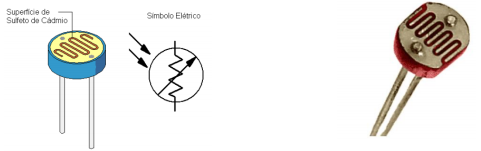
\includegraphics[width=0.9\linewidth]{Figuras/Ch03/fig16.PNG}}
}

\frame{
\frametitle{Sensores fotoelétricos}
\begin{block}{Curva característica do LDR}
A resistência elétrica do LDR decai à medida que a intensidade luminosa aumenta. 
\end{block}
\vspace{0.2cm}
\centerline{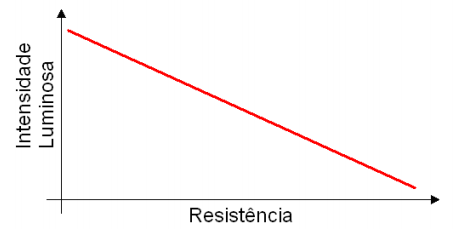
\includegraphics[width=0.6\linewidth]{Figuras/Ch03/fig17.PNG}}
}

\frame{
\frametitle{Sensores fotoelétricos}
\begin{block}{LDR}
\textbf{Vantagens}:
\begin{itemize}
    \item Podem operar com correntes relativamente altas, sendo muito sensíveis.
    \item Fácil utilização.
    \item Baixo preço.
\end{itemize}
\vspace{0.3cm}
\textbf{Desvantagem}:
\begin{itemize}
    \item Baixa velocidade de resposta - eles são sensores lentos.
\end{itemize}
\end{block}
}

\frame{
\frametitle{Sensores fotoelétricos}
\begin{block}{Fotocélula}
São dispositivos que geram uma pequena tensão elétrica quando são iluminados. As fotocélulas podem ser usadas para gerar energia elétrica a
partir da energia solar, ou também como sensores.
\end{block}
\vspace{0.2cm}
\centerline{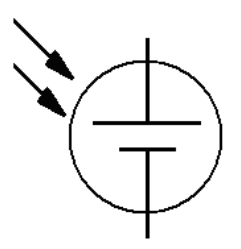
\includegraphics[width=0.3\linewidth]{Figuras/Ch03/fig18.PNG}}
}

\frame{
\frametitle{Sensores fotoelétricos}
\begin{block}{Fotocélula}
Uma aplicação possível é acionar o conjunto de iluminação de um estacionamento em função da diminuição da claridade do dia.
\end{block}
\vspace{0.2cm}
\centerline{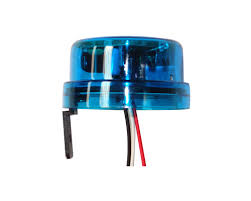
\includegraphics[width=0.5\linewidth]{Figuras/Ch03/fig19.jpg}}
}

\frame{
\frametitle{Sensores fotoelétricos}
\begin{block}{Fotocélula}
\textbf{Vantagens}:
\begin{itemize}
    \item Rápidas e sensíveis.
    \item Podem ser utilizadas em uma ampla faixa de aplicações.
    \item Fáceis de usar.
\end{itemize}
\vspace{0.3cm}
\textbf{Desvantagem}:
\begin{itemize}
    \item Podem ser imprecisas.
\end{itemize}
\end{block}
}

\frame{
\frametitle{Sensores térmicos}
\begin{block}{Introdução}
Para uma medição contínua de uma faixa de temperatura é preciso utilizar elementos \textbf{transdutores} que transformem esta informação em um outro sinal correspondente, tipicamente sinais de tensão de pequena amplitude (milivoltagem) ou variações de resistência.
\end{block}
}

\frame{
\frametitle{Sensores térmicos}
\begin{block}{Termopares}
É composto de \textbf{dois fios de metais diferentes unidos em uma das pontas}. Quando a ponta dos fios unidos está sob uma \textbf{temperatura diferente} da outra extremidade do termopar há uma tensão elétrica (da ordem de mV) provocada pela diferença de temperatura.
\end{block}
\centerline{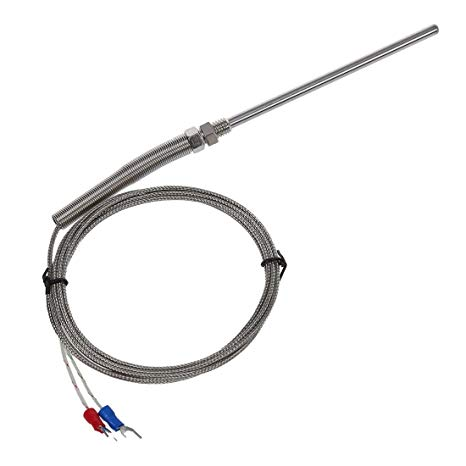
\includegraphics[width=0.4\linewidth]{Figuras/Ch03/fig20.jpg}}
}

\frame{
\frametitle{Sensores térmicos}
\begin{block}{Termopares}
\textbf{Vantagens}:
\begin{itemize}
    \item O diâmetro e o fio não influenciam no potencial gerado.
    \item O tempo de resposta é menor do que qualquer outro medidor de temperatura.
\end{itemize}
\vspace{0.3cm}
\textbf{Desvantagens}:
\begin{itemize}
    \item Eles podem sofrer a corrosão, especialmente quando expostos à temperatura limite superior.
    \item O sinal de saída é dado em milivolt (mV) sendo necessário um aparelho muito sensível para detectá-la.
\end{itemize}
\end{block}
}

\frame{
\frametitle{Sensores térmicos}
\begin{block}{Termistores}
Os sensores \textbf{NTC} e \textbf{PTC} também conhecidos como termistores, são tipos de sensores em que a \textbf{relação entre resistência elétrica e a temperatura} é conhecida. Operam em faixas de temperatura que vão de valores negativos até
aproximadamente $\SI{125}{\degree}$.
\end{block}
\centerline{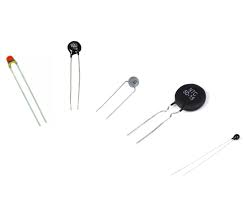
\includegraphics[width=0.6\linewidth]{Figuras/Ch03/fig21.jpg}}
}

\frame{
\frametitle{Sensores térmicos}
\centerline{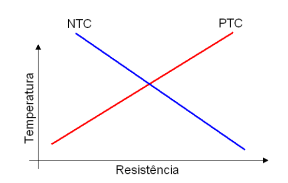
\includegraphics[width=0.7\linewidth]{Figuras/Ch03/fig22.PNG}}
}

\frame{
\frametitle{Sensores térmicos}
\begin{block}{Termistores}
\textbf{Vantagens}:
\begin{itemize}
    \item Grande faixa de aplicações, devido sua versatilidade e baixo custo.
    \item Boa tolerância e precisão.
\end{itemize}
\vspace{0.3cm}
\textbf{Desvantagens}:
\begin{itemize}
    \item Não linearidade.
    \item Inadequação para uso em temperaturas extremas.
\end{itemize}
\end{block}
}

\frame{
\frametitle{Sensores capacitivos}
\begin{block}{}
\textbf{Os sensores de proximidade capacitivos são semelhantes aos sensores de proximidade indutivos} em tamanho, forma e conceito. Entretanto, enquanto os sensores indutivos usam campos magnéticos indutivos para detectar objetos, os sensores de proximidade
capacitivos reagem às alterações do campo
eletrostático, por meio da \textbf{mudança da capacitância da placa detectora} localizada na região denominada face sensível.
\begin{itemize}
    \item Detecção capacitiva é uma tecnologia própria para detectar \textbf{não metais, sólidos e líquidos}. Pode detectar
    \textbf{metais}, porém o custo é mais elevado que o indutivo.
\end{itemize}
\end{block}
\centerline{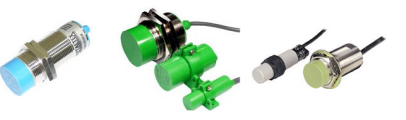
\includegraphics[width=0.7\linewidth]{Figuras/Ch03/fig23.PNG}}
}

\frame{
\frametitle{Sensores capacitivos}
\begin{block}{Aplicação}
Detecção de produto através da embalagem
\end{block}
\centerline{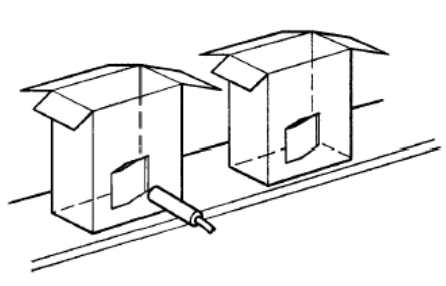
\includegraphics[width=0.7\linewidth]{Figuras/Ch03/fig24.PNG}}
}

\frame{
\frametitle{Sensores capacitivos}
\begin{block}{}
\textbf{Vantagens}:
\begin{itemize}
    \item Detectam metais e não metais, líquidos e sólidos.
    \item  Podem ``ver através'' de certos materiais (caixas de produto).
    \item Alta vida útil.
\end{itemize}
\vspace{0.3cm}
\textbf{Desvantagens}:
\begin{itemize}
    \item Distância sensora curta.
    \item Muito sensível aos fatores ambientais.
\end{itemize}
\end{block}
}

\frame{
\frametitle{Sensores ultrassônicos}
\begin{block}{}
É um tipo de sensor muito útil na detecção de objetos a uma certa distância, desde que não sejam muito pequenos, para que consigam \textbf{refletir as ondas sonoras}.
\begin{itemize}
    \item Um oscilador \textbf{emite ondas ultrassônicas} (em torno de 42 Khz), que resultam num comprimento de onda da ordem de alguns centímetros, o que permite detectar objetos relativamente pequenos. As ondas refletidas pelo objeto são capitadas pelo sensor, e o \textbf{tempo de resposta é proporcional à distância do objeto}.
\end{itemize}
\end{block}
\centerline{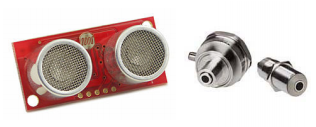
\includegraphics[width=0.7\linewidth]{Figuras/Ch03/fig25.PNG}}
}

\frame{
\frametitle{Sensores ultrassônicos}
\begin{block}{Aplicação}
Medição de nível em tanques
\end{block}
\centerline{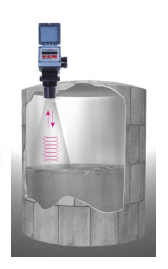
\includegraphics[width=0.3\linewidth]{Figuras/Ch03/fig26.PNG}}
}

\frame{
\frametitle{Sensores ultrassônicos}
\begin{block}{}
\textbf{Vantagens}:
\begin{itemize}
    \item Detectam objetos transparentes, nível de líquido ou superfícies altamente refletivas ou metálicas.
    \item Funcionam bem em ambientes úmidos.
\end{itemize}
\vspace{0.3cm}
\textbf{Desvantagens}:
\begin{itemize}
    \item São suscetíveis a flutuações de temperatura ou vento.
    \item Qualquer ruído acústico na frequência em que o sensor ultrassônico está recebendo pode interferir no desempenho desse sensor. 
\end{itemize}
\end{block}
}

\section*{Referências}
\frame{
\frametitle{Referências e Exercícios Complementares}
\begin{itemize}
\item THOMAZINI, D; ALBUQUERQUE, P. U. B. Sensores Industriais - Fundamentos e Aplicações. 5 ed. São Paulo: Érica, 2005.
\end{itemize}
%\centering{\alert{Página 546 - \textbf{Capítulo 6}}} \\
%\centering{\alert{Lista de exercícios 01}}
}

\frame{
\frametitle{Atuadores}
\begin{block}{Introdução}
\begin{itemize}
    \item São componentes que convertem energia elétrica, hidráulica ou pneumática em \textbf{energia mecânica}.
    \item Através dos sistemas de transmissão, a energia mecânica gerada pelos atuadores é enviada aos links do manipulador para que \textbf{se movimentem}.
    \item Deste modo, podemos definir um atuador como um \textbf{dispositivo destinado a executar uma ação}, como por exemplo, ligação de um motor; movimentação de uma esteira; abertura/fechamento de uma válvula; dosagem de material; etc.
\end{itemize}
\end{block}
}

\frame{
\frametitle{Atuadores}
\begin{block}{Atuadores hidráulicos}
\begin{itemize}
    \item São acionados por \textbf{fluidos em movimento}. Neste caso, o fluido é geralmente \textbf{óleo pressurizado}.
    \item Podem ter a forma de \textbf{cilindros lineares} para gerar os movimentos lineares ou \textbf{cilindros rotativos} para proporcionar deslocamentos angulares.
    \item São conectados a válvulas direcionais, que gerenciam a \textbf{direção do deslocamento} do fluido nos atuadores, a partir de sinais gerados por uma unidade de controle. O custo das válvulas direcionais de alto desempenho ainda é muito elevado.
\end{itemize}
\end{block}
}

\frame{
\frametitle{Atuadores}
\begin{block}{Atuadores hidráulicos}
\begin{itemize}
    \item Permitem a implementação de \textbf{controle contínuo e preciso de posicionamento e velocidade}, devido à incompressibilidade do fluido (óleo hidráulico), resultado numa elevada rigidez. Porém, isso torna \textbf{instável o controle da força}.
    \item Outra característica é a elevada relação entre a potência mecânica transmitida pelo atuador e seu peso, o que possibilita a \textbf{construção de unidades compactas de alta potência}.
    \item Uma bomba fornece o óleo para o atuador através das válvulas direcionais.
\end{itemize}
\end{block}
}

\frame{
\frametitle{Atuadores}
\centerline{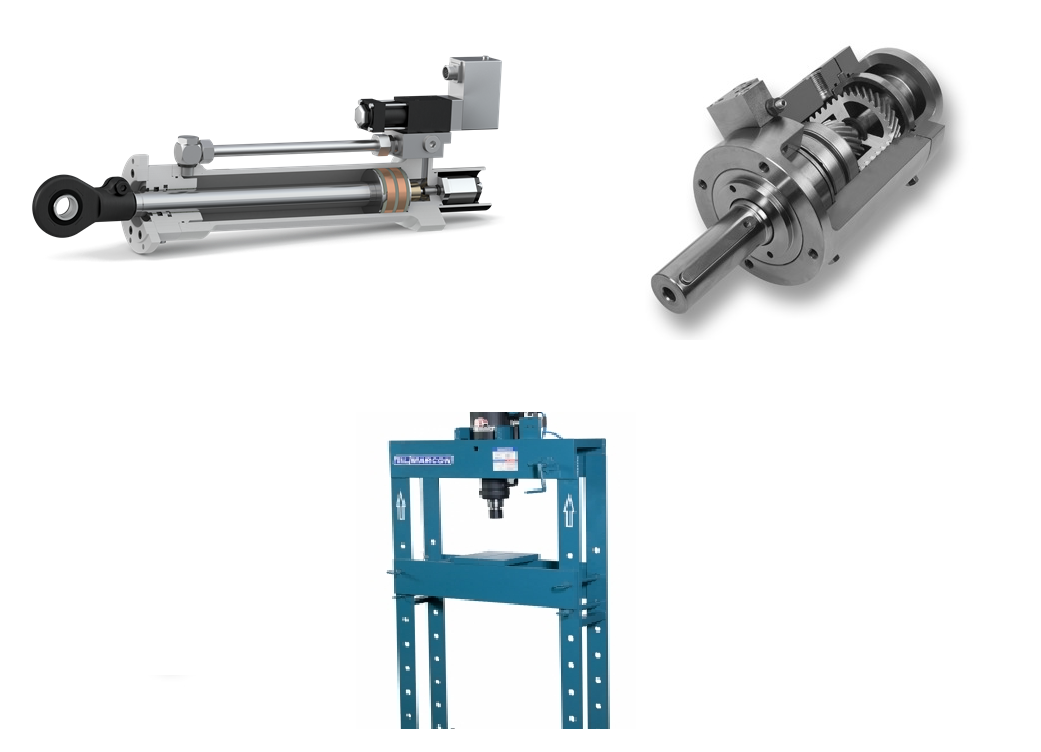
\includegraphics[width=0.9\linewidth]{Figuras/Ch03/fig27.jpg}}
}


\frame{
\frametitle{Atuadores}
\begin{block}{Atuadores pneumáticos}
\begin{itemize}
    \item São acionados por \textbf{fluidos em movimento}. Neste caso, o fluido é geralmente \textbf{ar comprimido}.
    \item Podem ter a forma de \textbf{cilindros lineares} para gerar os movimentos lineares ou \textbf{cilindros rotativos} para proporcionar deslocamentos angulares.
    \item São conectados a válvulas direcionais, que gerenciam a \textbf{direção do deslocamento} do fluido nos atuadores, a partir de sinais gerados por uma unidade de controle. O custo das válvulas direcionais de alto desempenho ainda é muito elevado.
\end{itemize}
\end{block}
}

\frame{
\frametitle{Atuadores}
\begin{block}{Atuadores pneumáticos}
\begin{itemize}
    \item Utilizados em \textbf{robôs industriais} que operam com movimentação de cargas entre posições bem definidas, limitadas por batentes mecânicos.
    \item Devido à \textbf{compressibilidade do fluido} (ar comprimido) possuem \textbf{baixa rigidez}.
    \item Permite que sejam obtidas operações suaves, porém com \textbf{pouca precisão} quanto ao controle de posicionamento entre as posições-limites.
    \item A natureza binária do movimento de cilindros pneumáticos (estendido ou retraído) implica em um \textbf{controle simples e de baixo custo}.
    \item Utiliza um \textbf{compressor} para fornecer o ar comprimido ao atuador pneumático, através das válvulas direcionais.
    \item Para correto funcionamento dos atuadores, recomenda-se a \textbf{instalação de unidades de preparação} (filtro, dreno, regulador de pressão, etc.) no circuito de ar comprimido, antes das válvulas direcionais.
\end{itemize}
\end{block}
}

\frame{
\frametitle{Atuadores}
\centerline{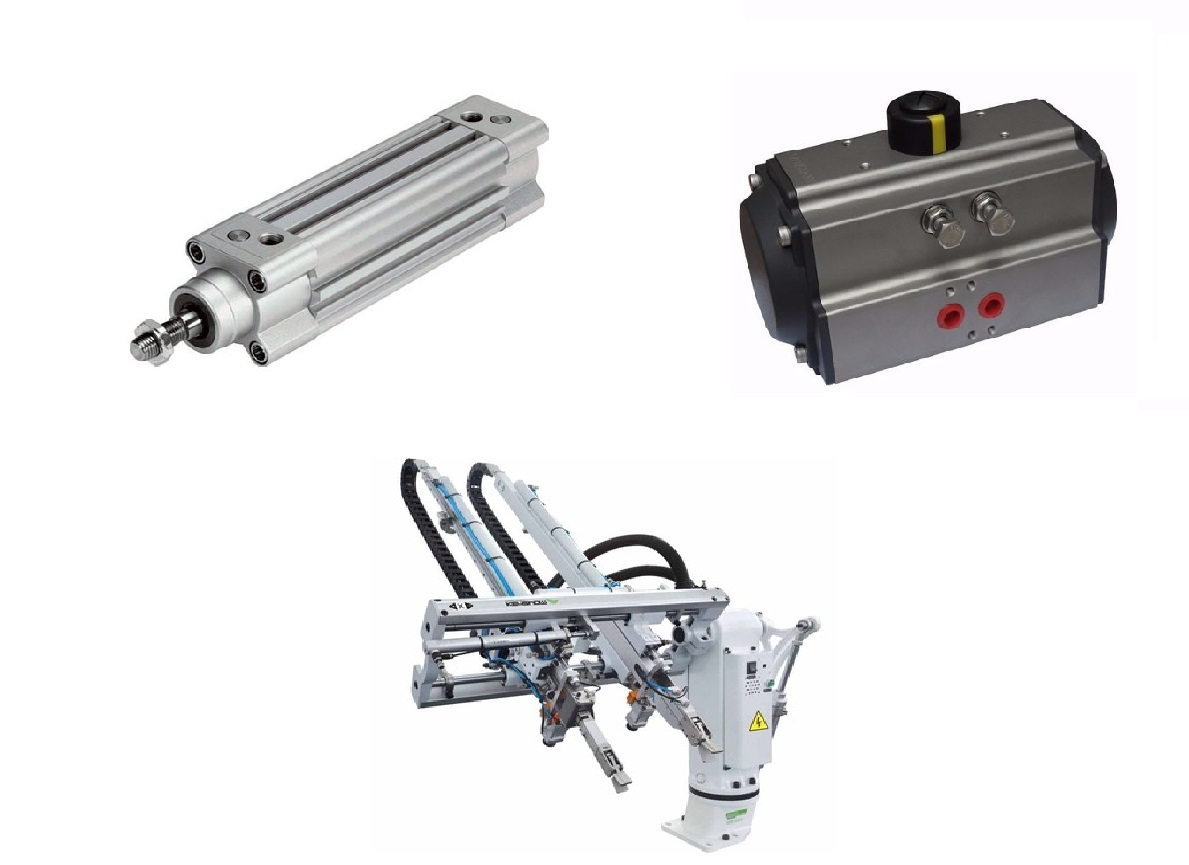
\includegraphics[width=0.9\linewidth]{Figuras/Ch03/fig28.jpg}}
}

\frame{
\frametitle{Atuadores}
\begin{block}{Atuadores eletromagnéticos}
\begin{itemize}
    \item São os atuadores mais utilizados em robôs, principalmente os \textbf{motores C.C.} e os \textbf{motores de passo}.
    \item Possuem as seguintes \textbf{vantagens}: grande variedade de fabricantes e modelos no mercado; motores elétricos, quando associados a sensores, podem ser empregados tanto pra o controle de força quando para o controle de posição do robô; são mais fáceis de programar seus movimentos, já que podem ser controlados por sinais elétricos, permitindo a utilização de controladores de movimento; etc.
\end{itemize}
\end{block}
}

\frame{
\frametitle{Atuadores}
\begin{block}{Atuadores eletromagnéticos - motores de C.C.}
\begin{itemize}
    \item São \textbf{compactos} e geralmente mantém o valor de torque numa faixa constante para grandes variações de velocidade.
    \item \textbf{Necessitam de sensores de posição e de velocidade}, para controle de posicionamento em malha fechada (servocontrole).
    \item A máxima eficiência mecânica desses motores normalmente ocorre a velocidade elevadas, por isso é comum o uso de \textbf{redutores}.
\end{itemize}
\end{block}
}

\frame{
\frametitle{Atuadores}
\centerline{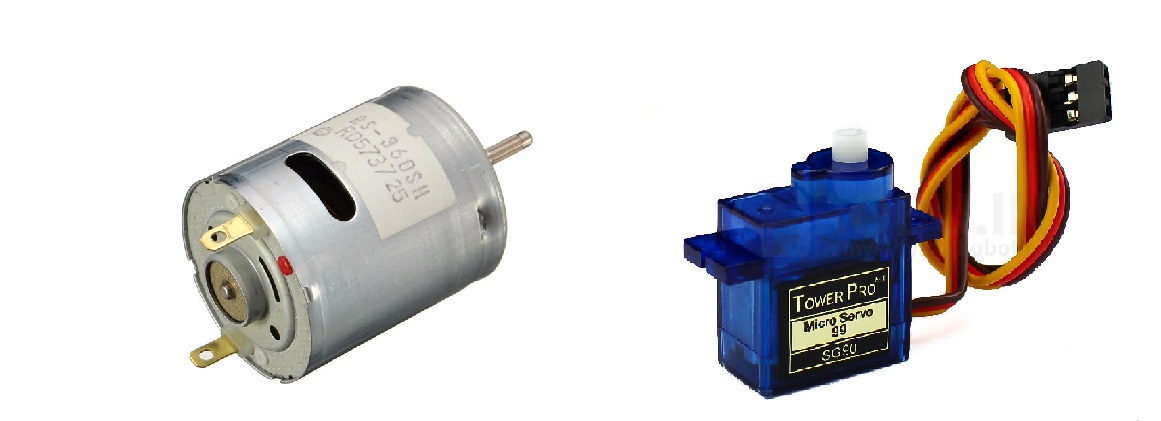
\includegraphics[width=0.9\linewidth]{Figuras/Ch03/fig29.jpg}}
}

\frame{
\frametitle{Atuadores}
\begin{block}{Atuadores eletromagnéticos - motores de passo}
\begin{itemize}
    \item É essencialmente um motor C.C., mas com um \textbf{controle sobre o deslocamento do eixo}. Cada deslocamento angular é chamado de \textbf{passo}.
    \item Podem funcionar em controle de malha aberta, em posição e velocidade, e são facilmente interligados a \textbf{unidades de controle simples e de baixo custo}.
    \item Entretanto, no motores de passo a curva de torque decresce com o aumento de velocidade e, \textbf{em baixas velocidades, podem gerar vibrações mecânicas}.
    \item Em robótica, são mais empregados na \textbf{movimentação de garras}.
    \item O ponto forte de um motor de passo não é a sua força (torque), tampouco sua capacidade de desenvolver altas velocidades - ao contrário da maioria dos outros motores elétricos - mas sim a possibilidade de
    \textbf{controlar seus movimentos de forma precisa}. 
\end{itemize}
\end{block}
}

\frame{
\frametitle{Atuadores}
\centerline{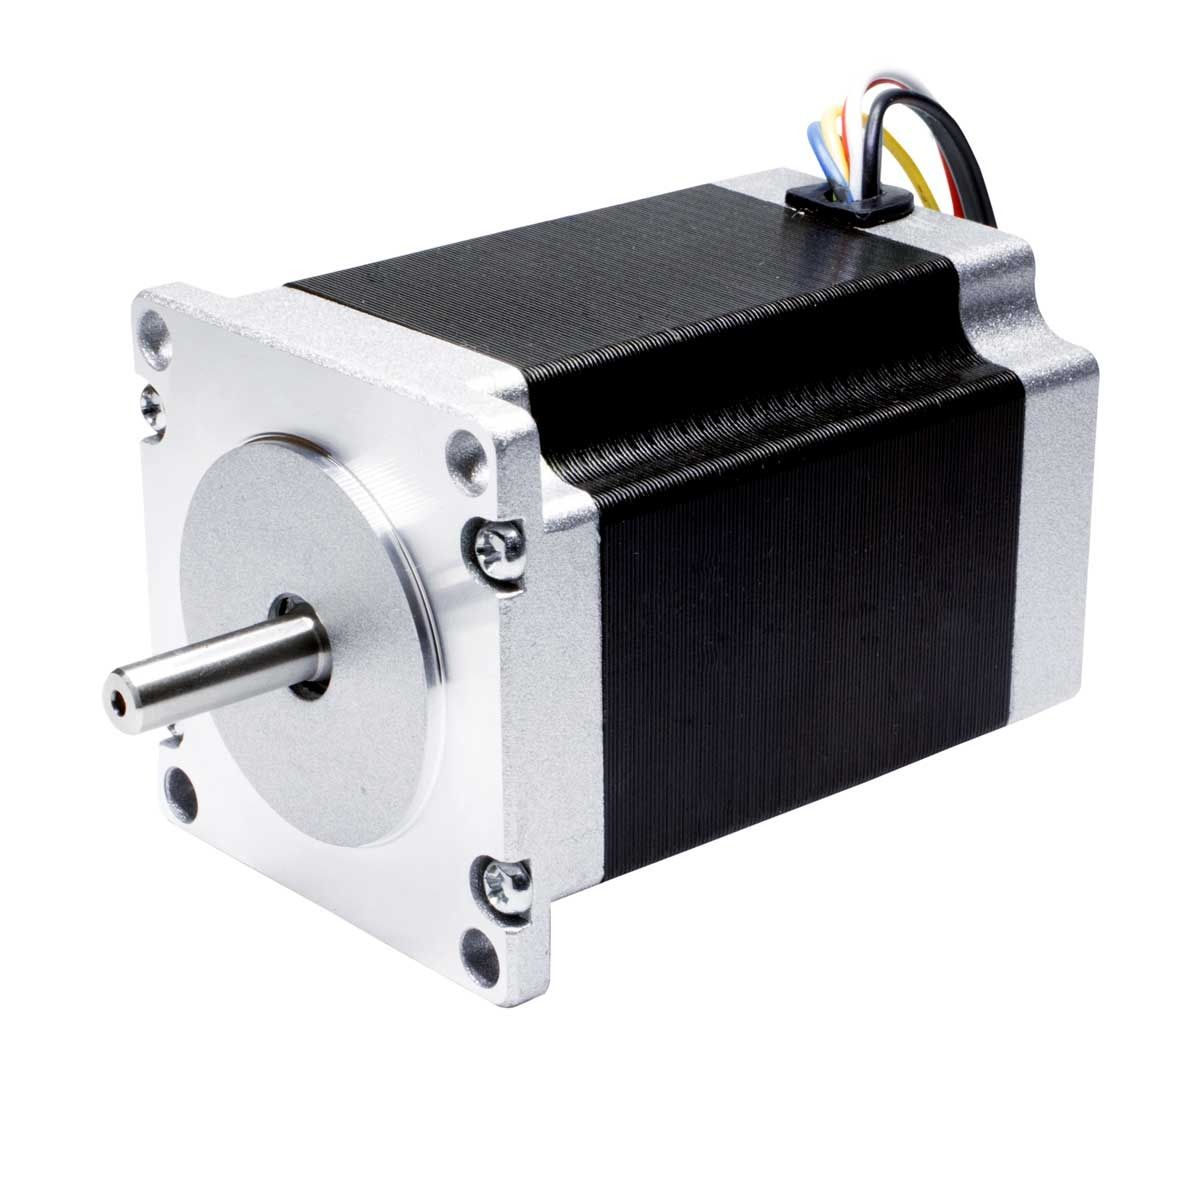
\includegraphics[width=0.5\linewidth]{Figuras/Ch03/fig30.jpg}}
}

\frame{
\frametitle{Atuadores}
\begin{tabular}{ccc}
	\toprule
	\textbf{Hidráulicos} & \textbf{Pneumáticos} & \textbf{Eletromagnéticos} \\ \midrule
	\makecell{Transporte de cargas \\ pesadas} &
	\makecell{Transporte de cargas \\ pequenas e médias} &
	\makecell{Transporte de cargas \\ pequenas e médias} \\ [0.3cm]
	\makecell{Precisão média-alta \\ no controle de posição e \\ velocidade} & Baixa precisão & Alta precisão \\ [0.2cm]
	& \makecell{Altas velocidades e \\ baixo custo}&  Ocupa pouco espaço \\ \bottomrule
\end{tabular}
}

\section*{Referências}
\frame{
\frametitle{Referências e Exercícios Complementares}
\begin{itemize}
\item NATALE, F. Automação Industrial. 10 ed. São Paulo: Érica, 2013.
\end{itemize}
%\centering{\alert{Página 546 - \textbf{Capítulo 6}}} \\
%\centering{\alert{Lista de exercícios 01}}
}